\documentclass[tikz,border=2pt]{standalone}
\usepackage{pgfplots}
\usetikzlibrary{intersections}
\usepgfplotslibrary{fillbetween}
\pgfplotsset{compat=1.7}
\pgfplotsset{
    legend image with text/.style={
        legend image code/.code={%
            \node[anchor=center] at (0.3cm,0cm) {#1};
        }
    },
}


\begin{document}
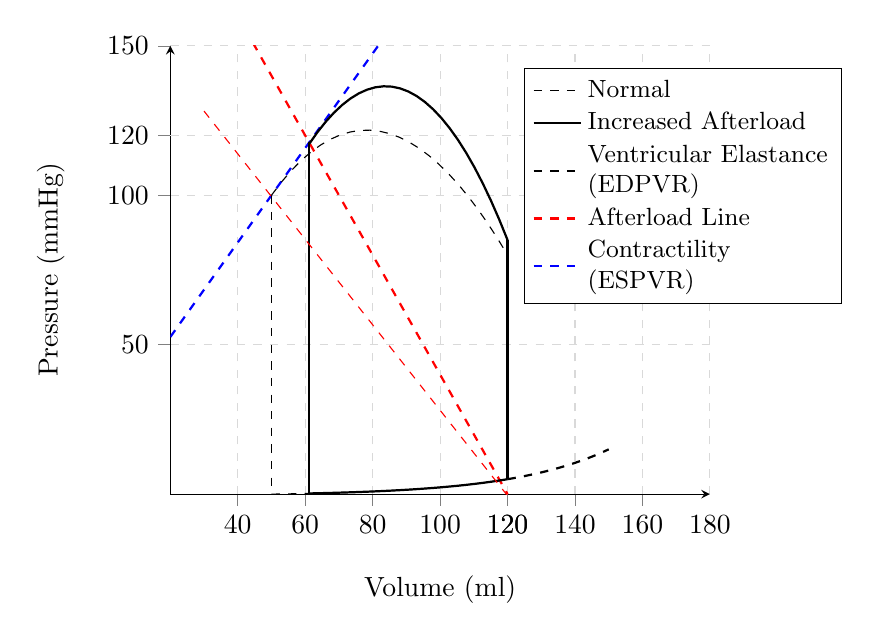
\begin{tikzpicture}



\begin{axis}[
        axis lines=middle,
        grid = major,
        grid style={dashed, gray!30},
	ymin = 0,
	ymax = 150,
	xmin = 20,
	xmax =180,
	 ylabel near ticks,
	xlabel near ticks,
	extra y ticks={120},
	extra x ticks={120},
        xlabel=Volume (ml),
        ylabel=Pressure (mmHg),
        tick align=outside,
        enlargelimits=false,
	legend pos= north west,
	legend style={font=\small, cells={align=left}, at={(0.95,0.95)},anchor=north},
legend cell align={left}]

\node (o) at (axis cs: 0,0){};

%ESPVR and Afterload lines
\addplot[name path=afterload,red, thick, dashed, domain=30:120, forget plot] {-2*x+240};
\addplot[name path=contractility,blue, thick, dashed, domain=0:100, forget plot] {1.581*x+20.95};

\path [name intersections={of=contractility and afterload,by=A}];


%EDPVR
\addplot[name path=bot, black, thick, domain=61.17:120, forget plot] {-0.400992 - (-0.002991122/-0.03458544)*(1 - e^(+0.03458544*x))};
\addplot[black, thick, dashed, domain=120:150, forget plot] {-0.400992 - (-0.002991122/-0.03458544)*(1 - e^(+0.03458544*x))};

%IVC
\draw[black,thick] (axis cs: 120,5) -- (axis cs: 120,85);

%Ejection
\addplot[name path=top, black, thick, domain=61.17:120, forget plot] {-115.6429 + 5.814269*x - 0.03108155*x^2 - 0.00002864296*x^3};

%IVR
\draw[black, thick] (A) -- (A|-o);


%normal loop
\addplot[name path=bot, black, thin, dashed, domain=50:120, forget plot] {-0.400992 - (-0.002991122/-0.03458544)*(1 - e^(+0.03458544*x))};
\draw[black,thin, dashed] (axis cs: 120,5) -- (axis cs: 120,80);
\addplot[name path=top, black, thin, dashed, domain=50:120, forget plot] {-60 + 4.938095*x - 0.03714286*x^2 + 0.00004761905*x^3};
\draw[black, thin, dashed] (axis cs: 50,100) -- (axis cs: 50,0);
\addplot[red, thin, dashed, domain=30:120, forget plot] {-1.43*x+171.06};

%legend
\addlegendimage{black, thin, dashed};
\addlegendentry{Normal};
\addlegendimage{black, thick};
\addlegendentry{Increased Afterload};
\addlegendimage{black, dashed, thick};
\addlegendentry{Ventricular Elastance \\ (EDPVR)}
\addlegendimage{red, dashed, thick};
\addlegendentry{Afterload Line}
\addlegendimage{blue, dashed, thick};
\addlegendentry{Contractility \\ (ESPVR)}



\end{axis}

\end{tikzpicture} 
\end{document}